\renewcommand\appendixpagename{Bijlagen}
\renewcommand\appendixtocname{Bijlagen}

\begin{appendices}
    \chapter{Assets.json}    
    \label{app:assetsjson}
    \lstset{language=JSON}
    \begin{lstlisting}
    {
        "common": [{
            "src": "assets/language/PDALanguage.lp",
            "id": "language"
        }],
        "scenario_test_movie": [{
                "src": "assets/scenarios/scenario_test_movie/story.json",
                "id": "story_scenario_test_movie"
            },
            {
                "src": "assets/scenarios/scenario_test_movie/story.lp",
                "id": "story_scenario_test_movie.lp"
            }
        ],
        "scenario_test_movie_lazyLoad": [{
                "src": "assets/scenarios/scenario_test_movie/images/JF_Angry.jpg",
                "id": "JF_Angry_jpg"
            },
            {
                "src": "assets/scenarios/scenario_test_movie/images/JF_Angry.png",
                "id": "JF_Angry_png"
            },
            {
                "src": "assets/scenarios/scenario_test_movie/images/JF_Sad.jpg",
                "id": "JF_Sad_jpg"
            },
            {
                "src": "assets/scenarios/scenario_test_movie/images/JF_Sad.png",
                "id": "JF_Sad_png"
            }
        ],
        "sounds": [{
                "src": "assets/sounds/click.mp3",
                "id": "click"
            },
            {
                "src": "assets/sounds/counter_1.mp3",
                "id": "counter"
            },
            {
                "src": "assets/sounds/drill.mp3",
                "id": "drill"
            },
    
            {
                "src": "assets/sounds/pda/smartphone_open.mp3",
                "id": "smartphone_open"
            },
            {
                "src": "assets/sounds/pda/smartphone_close.mp3",
                "id": "smartphone_close"
            },
            {
                "src": "assets/sounds/pda/smartphone_clickbutton.mp3",
                "id": "smartphone_clickbutton"
            }
        ]
    }
    \end{lstlisting}

    \chapter{Voorbeeld content typen schema}
    \lstset{language=JSON}
    \begin{lstlisting}
    {
        "$schema": "http://json-schema.org/draft-07/schema#",
        "$id": "http://www.ranjnet.nl/ozcontent#",
        "title": "&ranj game content",
        "description": "This schema defines the content types within the game content",
        "definitions": {
            "propertyTypes": {
                "stringProperty": {
                    "$id": "#/definitions/propertyTypes/stringProperty",
                    "type": "string",
                    "default": ""
                },
                "booleanProperty": {
                    "$id": "#/definitions/propertyTypes/booleanProperty",
                    "type": "boolean",
                    "default": false
                },
                "resourceProperty": {
                    "$id": "#/definitions/propertyTypes/resourceProperty",
                    "type": "string"
                },
                "variableMutationProperty": {
                    "$id": "#/definitions/propertyTypes/variableMutationProperty",
                    "type": "object",
                    "properties": {
                        "variableKey": {
                            "$ref": "#/definitions/propertyTypes/stringProperty"
                        },
                        "mutationType": {
                            "$ref": "#/definitions/propertyTypes/stringProperty",
                            "enum": [
                                "Set",
                                "Add",
                                "Subtract",
                                "Multiple",
                                "Divide"
                            ],
                            "default": "Set"
                        },
                        "mutationValue": {
                            "$ref": "#/definitions/propertyTypes/stringProperty"
                        }
                    }
                }
            },
            "baseContent": {
                "type": "object",
                "properties": {
                    "contentType": {
                        "$ref": "#/definitions/propertyTypes/stringProperty"
                    },
                    "label": {
                        "$ref": "#/definitions/propertyTypes/stringProperty",
                        "title": "Label"
                    },
                    "retained": {
                        "$ref": "#/definitions/propertyTypes/booleanProperty",
                        "title": "Retained"
                    },
                    "contentID": {
                        "$ref": "#/definitions/propertyTypes/stringProperty",
                        "title": "Content ID"
                    }
                },
                "required": [
                    "type",
                    "label",
                    "retained",
                    "contentID"
                ]
            }
        },
        "contentTypes": {
            "textContent": {
                "allOf": [{
                        "$ref": "#/definitions/baseContent"
                    },
                    {
                        "$id": "#/contentTypes/textContent",
                        "title": "Text content",
                        "description": "Textual content",
                        "properties": {
                            "text": {
                                "allOf": [{
                                        "$ref": "#/definitions/propertyTypes/stringProperty"
                                    },
                                    {
                                        "title": "Text",
                                        "description": "Value of the textual content"
                                    }
                                ]
                            }
                        }
                    }
                ]
            },
            "imageContent": {
                "allOf": [{
                        "$ref": "#/definitions/baseContent"
                    },
                    {
                        "$id": "#/contentTypes/imageContent",
                        "title": "Image content",
                        "properties": {
                            "imageResource": {
                                "allOf": [{
                                        "$ref": "#/definitions/propertyTypes/resourceProperty"
                                    },
                                    {
                                        "assetType": "image"
                                    }
                                ]
                            }
                        }
                    }
                ]
            },
            "variableMutationContent": {
                "allOf": [{
                        "$ref": "#/definitions/baseContent"
                    },
                    {
                        "title": "Mutate variable content",
                        "$id": "#/contentTypes/variableMutationContent",
                        "properties": {
                            "mutations": {
                                "type": "array",
                                "items": {
                                    "$ref": "#/definitions/propertyTypes/variableMutationProperty"
                                }
                            }
                        }
                    }
                ]
            }
        }
    }
    \end{lstlisting}

    \chapter{Content typen dataschema in XML}
    \label{app:contenttypeschemeinxml}
    % \subsection*{XML-dataschema}
    XML heeft al ingebouwde dataschema functionaliteit; de onderliggende structuur van een XML-object kan worden gespecificeerd. Dit bereikt XML door middel van elementen en attributen. Zo kan ‘sms content’ worden beschreven in een XML-dataschema als in \autoref{fig:xmlschemasmscontent}. Vervolgens kunnen XML-objecten gevalideerd worden door het schema. Het XML-object in \autoref{fig:xmlsmscontent} is valide, want de structuur komt overeen met die van het dataschema in \autoref{fig:xmlschemasmscontent}.

    \begin{figure}[htb]
        \centering
        \lstset{
        language=XML,
        morekeywords={encoding,
            xs:schema,xs:element,xs:complexType,xs:sequence,xs:attribute}
        }
        \begin{lstlisting}
        <?xml version="1.0" encoding="UTF-8"?>
        <xs:schema xmlns:xs="http://www.w3.org/2001/XMLSchema">
            <xs:element name="smscontent">
                <xs:complexType>
                    <xs:sequence>
                        <xs:element name="sender" type="xs:string" />
                        <xs:element name="receiveDate" type="xs:dateTime" />
                        <xs:element name="content" type="xs:string" />
                    </xs:sequence>
                </xs:complexType>
            </xs:element>
        </xs:schema>                
        \end{lstlisting}
        \caption{XML-dataschema voor 'sms content'.}
        \label{fig:xmlschemasmscontent}
    \end{figure}

    \begin{figure}[htb]
        \centering
        \lstset{language=XML}
        \begin{lstlisting}[firstnumber=1]
        <?xml version="1.0" encoding="UTF-8"?>
        <smscontent>
            <sender>Harold</sender>
            <receiveDate>2018-04-21T11:00:00</receiveDate>
            <content>Great moves, keep it up!</content>
        </smscontent>              
        \end{lstlisting}
        \caption{Valide XML-object van 'sms content'.}
        \label{fig:xmlsmscontent}
    \end{figure}
    
    \chapter{Use cases voor een overkoepelende projectstructuur}
    \label{app:usecasesprojectstructuur}
    \begin{itemize}
        \item Als gebruiker wil ik kunnen kiezen uit een lijst van (gecategoriseerde) assets.
        \item Als gebruiker wil ik gewaarschuwd worden als ik een niet-bestaande of verkeerd type asset gebruik.
        \item Als gebruiker wil ik een preview kunnen zien of horen als mogelijk.
        \item Als gebruiker wil ik assets kunnen openen. (dialog/ story files openen in de editor, afbeeldingen met default afbeeldingen programma)
        \item Als gebruiker wil ik dat mijn game geen ongebruikte assets laadt. (Als speler wil ik dat mijn game snel laad).
        \item Als gebruiker wil ik gedeelde variabelen kunnen gebruiken in zowel het verhaal als dialoog.
    \end{itemize}

    \chapter{Balkenplanning}
    \label{app:ganttchart}
    \newcounter{myWeekNum}
    \stepcounter{myWeekNum}
    
    \newcommand{\myWeek}{\themyWeekNum
        \stepcounter{myWeekNum}
        \ifnum\themyWeekNum=6
            \setcounter{myWeekNum}{1}
        \else\fi
    }

    \setcounter{myWeekNum}{6}
    \ganttset{%
        calendar week text={\myWeek{}}%
    }
    % \ganttset{bar height=.6}

    % \begin{landscape}
    \begin{adjustwidth}{-0.7cm}{}
        \noindent\resizebox{1.1\textwidth}{!}{
            \begin{ganttchart}[
                hgrid,
                vgrid={*{6}{draw=none}, dotted},
                x unit=.08cm,
                y unit title=.6cm,
                y unit chart=.6cm,
                time slot format=isodate
                ]{2018-02-05}{2018-07-13}
                \gantttitlecalendar{year, month=name, week} \\
                % start of reoccurring items
                \ganttmilestone{Overleg met bedrijfsbegeleider}{2018-02-05}
                \ganttmilestone{}{2018-02-12}
                \ganttmilestone{}{2018-02-19}
                \ganttmilestone{}{2018-02-26}
                \ganttmilestone{}{2018-03-05}
                \ganttmilestone{}{2018-03-12}
                \ganttmilestone{}{2018-03-19}
                \ganttmilestone{}{2018-03-26}
                \ganttmilestone{}{2018-04-03}
                \ganttmilestone{}{2018-04-09}
                \ganttmilestone{}{2018-04-16}
                \ganttmilestone{}{2018-04-25}
                \ganttmilestone{}{2018-04-30}
                \ganttmilestone{}{2018-05-14}
                \ganttmilestone{}{2018-05-21}
                \ganttmilestone{}{2018-05-28}
                \ganttmilestone{}{2018-06-04} \\

                \ganttmilestone{Overleg met afstudeerbegeleider}{2018-02-19}
                \ganttmilestone{}{2018-03-05}
                \ganttmilestone{}{2018-03-19}
                \ganttmilestone{}{2018-04-09}
                \ganttmilestone{}{2018-05-07}
                \ganttmilestone{}{2018-05-22}
                \ganttmilestone{}{2018-06-04} \\
                
                \ganttbar{Werken aan prototype}{2018-03-19}{2018-03-25}
                \ganttbar{}{2018-04-09}{2018-04-15}
                \ganttbar{}{2018-04-26}{2018-05-06}
                \ganttbar{}{2018-06-19}{2018-07-04}
                \\

                \ganttbar{Documenteren}{2018-03-19}{2018-03-25}
                \ganttbar{}{2018-04-09}{2018-04-15}
                \ganttbar{}{2018-05-07}{2018-05-13}
                \ganttbar{}{2018-05-28}{2018-06-03}
                \\
                % end of reoccurring items

                % % initiatie
                \ganttgroup{Initiatie}{2018-02-05}{2018-03-04} \\
                \ganttbar{Initiatie \& oriëntatie}{2018-02-05}{2018-02-18} \\
                \ganttbar{Vragen in kaart brengen}{2018-02-19}{2018-03-04} \\
                \ganttbar{Requirements opstellen}{2018-02-19}{2018-03-04} \\
                
                % % technologieën
                \ganttgroup{Technologieën}{2018-03-05}{2018-03-25} \\
                \ganttbar{Tech stack van \&ranj inkaart brengen}{2018-03-05}{2018-03-08} \\
                \ganttbar{Requirements/ aandachtspunten opstellen}{2018-03-08}{2018-03-11} \\
                \ganttbar{Inventariseren bruikbare technologieën}{2018-03-12}{2018-03-18} \\
                % \ganttbar{Inventariseren ontwikkelplatformen}{2018.49}{2018.50} \\
                % \ganttbar{Inventariseren UI frameworks}{2018.49}{2018.50} \\
                % \ganttbar{Inventariseren diagramming libraries}{2018.49}{2018.50} \\
                % + prototype 2018-03-18 2018-03-25
                % + documenteren 2018-03-18 2018-03-25

                % % diversiteit in game content
                \ganttgroup{Diversiteit in game content}{2018-03-26}{2018-04-15} \\
                \ganttbar{Wat is game content}{2018-03-26}{2018-03-28} \\
                \ganttbar{Onderscheid maken tussen game content}{2018-03-29}{2018-04-01} \\
                \ganttbar{Inlezen dataschema's}{2018-04-02}{2018-04-08} \\
                \ganttbar{Toepassen dataschema's}{2018-04-09}{2018-04-15} \\
                % + prototype 2018-04-16 2018-04-22
                % + documenteren 2018-04-23 2018-04-29

                % % formalismen
                \ganttgroup{Formalismen}{2018-04-16}{2018-05-13} \\
                \ganttbar{Wat is formalisme}{2018-04-16}{2018-04-18} \\
                \ganttbar{Hoe gaan andere tools hier mee om}{2018-04-19}{2018-04-22} \\
                \ganttbar{Formalisme in de huidige editors}{2018-04-23}{2018-04-26} \\
                \ganttbar{Visuele representatie scheiden van formalisme}{2018-04-26}{2018-05-06} \\
                % + prototype 2018-05-04 2018-05-13
                % + documenteren 2018-05-14 2018-05-20
                
                % % overkoepelende projectstructuur
                \ganttgroup{Overkoepelende projectstructuur}{2018-05-14}{2018-06-03} \\
                \ganttbar{Huidige projectstructuur in kaart brengen}{2018-05-14}{2018-05-16} \\
                \ganttbar{Hoe kunnen bestanden worden beheerd}{2018-05-16}{2018-05-23} \\
                \ganttbar{Hoe kan semantiek worden gebonden aan bestanden}{2018-05-24}{2018-06-03} \\
                % + documenteren 2018-05-28 2018-06-03

                % % reflectie/ afronding
                \ganttgroup{Afsluiting}{2018-06-04}{2018-07-04} \\
                \ganttbar{Documenteren + eventuele reperatie}{2018-06-04}{2018-06-18} \\
                \ganttbar{Voorbereiding eindpresentatie}{2018-06-19}{2018-07-04}
                
                % % deadlines
                \ganttvrule[vrule label node/.append style={anchor=north east}
                ]{Concept}{2018-06-04}
                \ganttvrule{Deadline}{2018-06-18}
                \ganttvrule[vrule label node/.append style={anchor=north west}
                ]{Afstudeerzitting}{2018-07-04}
            \end{ganttchart}
        }
        \end{adjustwidth}
    % \end{landscape}

    \chapter{Competentiewijzer}
    \begin{figure}[htb]
        \begin{tabular}{ | l | l | }
            \hline
            \textbf{Competentie} & \textbf{Lokatie}\\
            \hline
            \multicolumn{2}{ | c | }{\textbf{Beheren}}\\
            \hline
            B1 & \autoref{app:ganttchart}\\% aansterken met tussentijdseplanning + reflectie?
            B2 & \autoref{app:getuigenverklaringen}\\
            \hline
            \multicolumn{2}{ | c | }{\textbf{Analyseren}}\\
            \hline
            AN1 & \autoref{sec:probleemstelling}, \autoref{sec:doelstelling}\\
            AN2 & \autoref{subsec:ontwikkelprocesnarrativegames}, \autoref{ch:technologystack}, \autoref{subsec:statischedefinities}, \autoref{app:usecasesprojectstructuur}\\
            AN3 & \autoref{sec:ontwikkelplatformen}, \autoref{subsec:uiframeworksandlibraries}, \autoref{subsec:diagramminglibraries}, \autoref{subsec:formulerenvanbouwblokken}, \autoref{subsec:hetcompilerenvaneenvisuelestructuur} \\
            AN4 & \autoref{sec:ontwikkelplatformen}, \autoref{subsec:uiframeworksandlibraries}, \autoref{subsec:diagramminglibraries}, \autoref{subsec:formulerenvanbouwblokken}, \autoref{app:contenttypeschemeinxml} \\
            \hline
            \multicolumn{2}{ | c | }{\textbf{Adviseren}}\\
            \hline
            AD1 & \autoref{ch:technologystack}, \autoref{sec:flexibeleselectiecontenttypen},  \\
            AD2 & \\
            AD3 & Zal blijken uit presentatie \\
            \hline
            \multicolumn{2}{ | c | }{\textbf{Ontwerpen}}\\
            \hline
            O1 & \\
            O2 & \\
            O3 & \\
            O4 & \\
            O5 & \\
            \hline
        \end{tabular}
        \centering
        \caption{Competentiewijzer; een map tussen competenties en waar deze potentieel bewezen worden.}
    \end{figure}

    % Getuigenverklaringen
    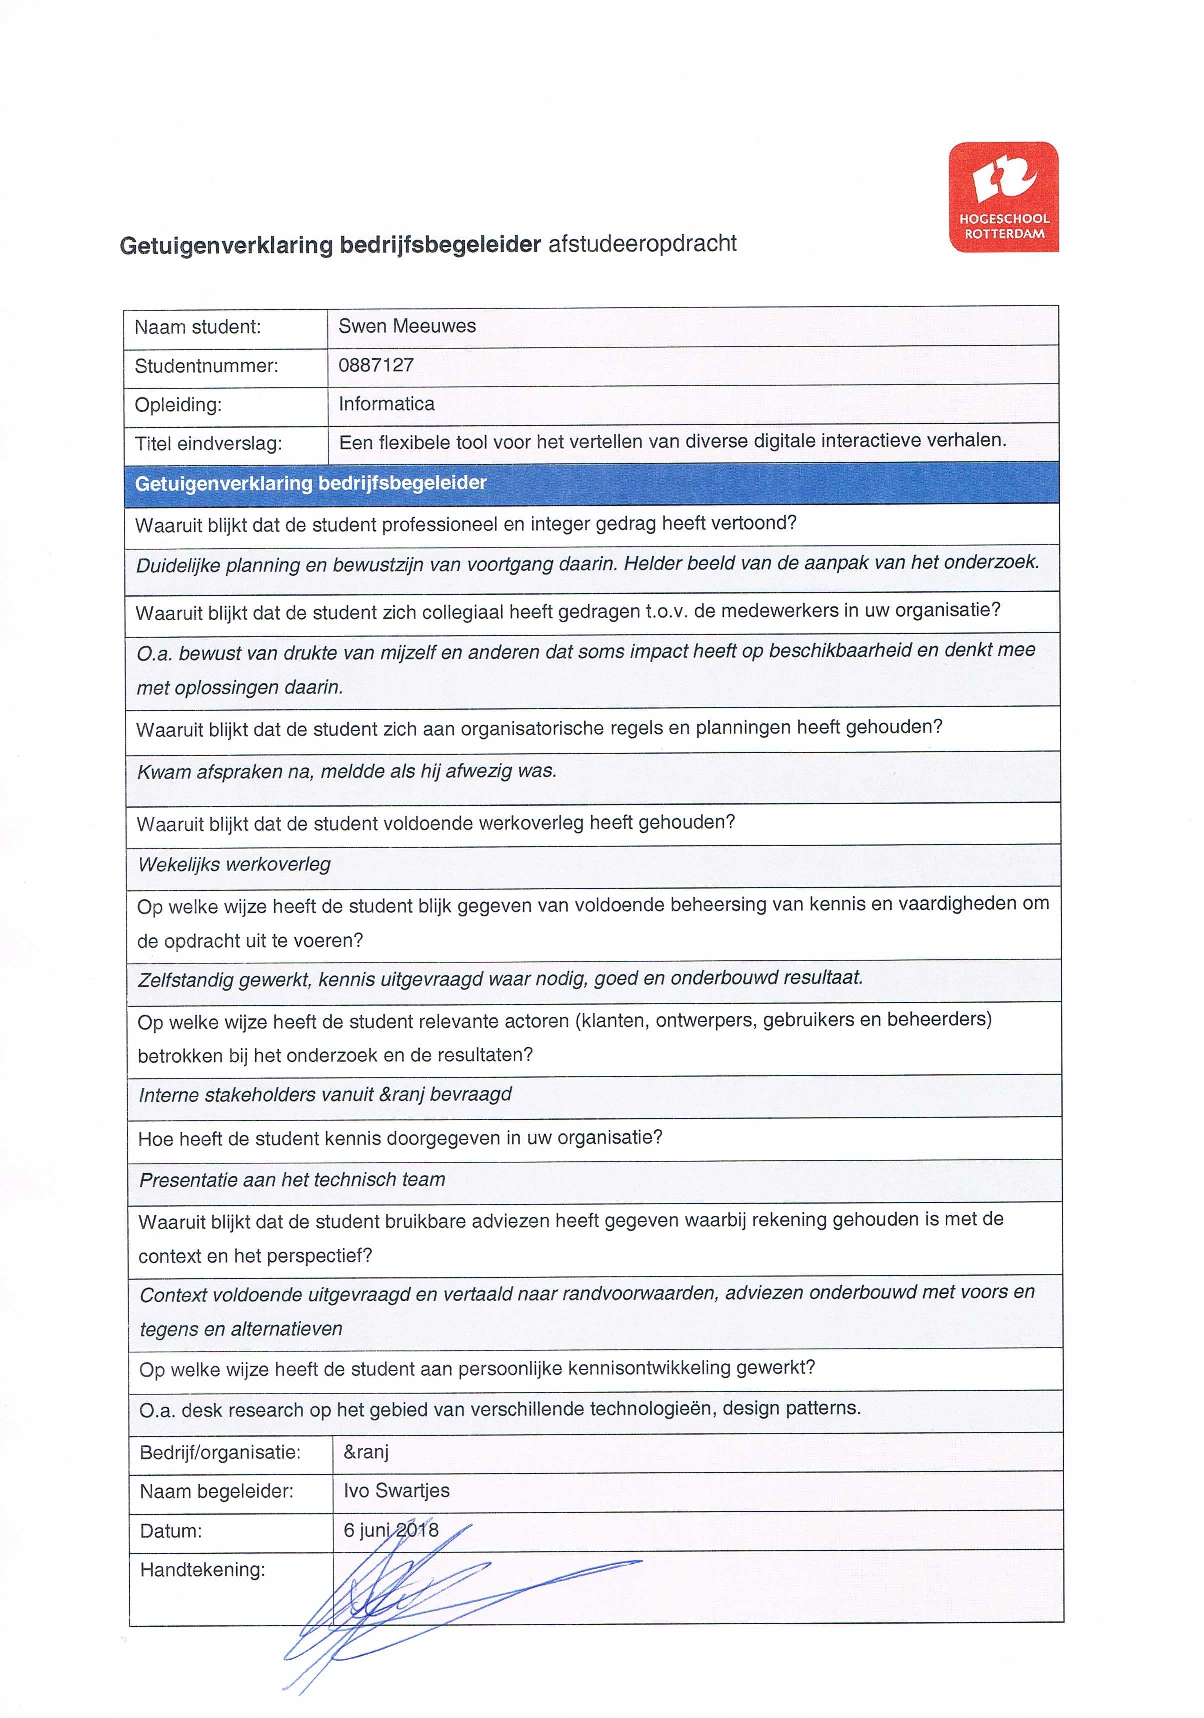
\includepdf[pages=-,scale=.75,offset=0mm -25mm,pagecommand=\chapter{Getuigenverklaringen}\label{app:getuigenverklaringen}]{assets/pdf/Getuigenverklaring_bedrijfsbegeleider.pdf}
    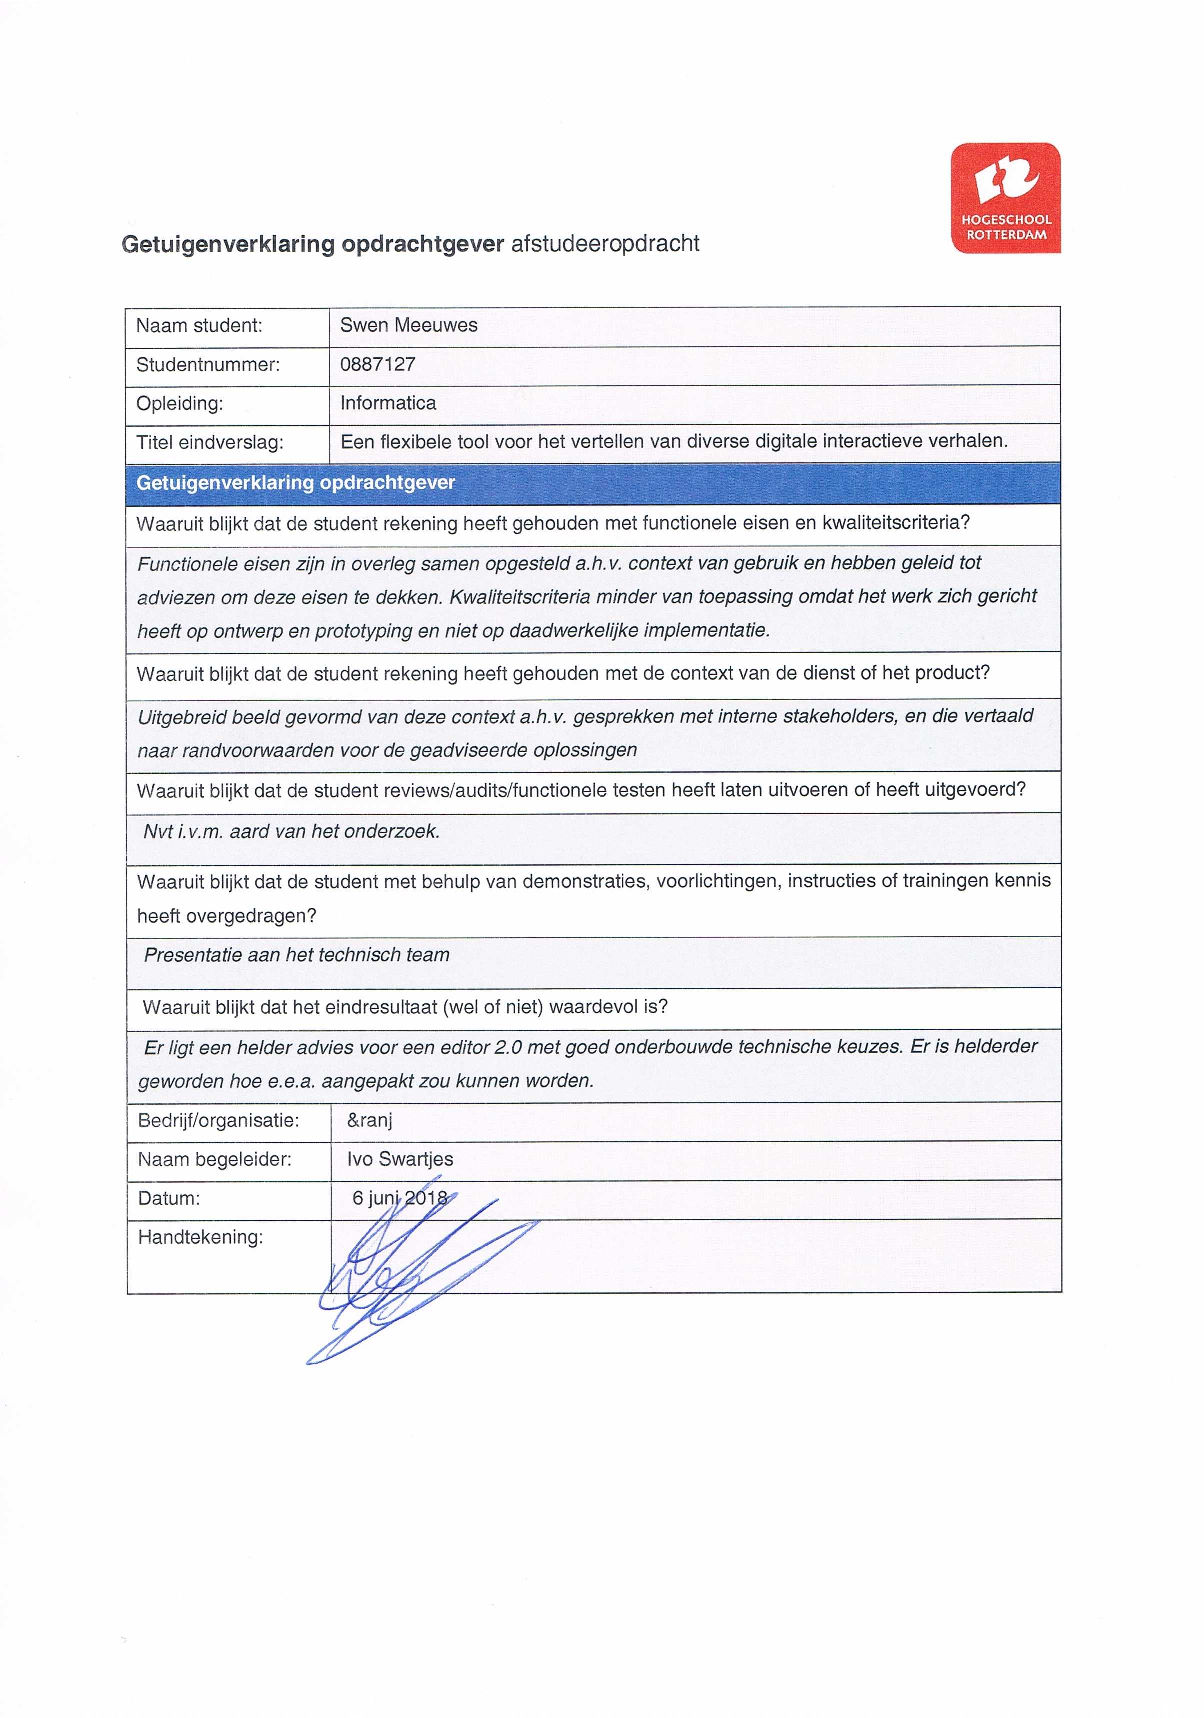
\includepdf[pages=-,scale=.75,pagecommand={}]{assets/pdf/Getuigenverklaring_opdrachtgever.pdf}
\end{appendices}